\subsection{Consultation des factures}
Cette section concerne la création et la consultation de factures ainsi que la génération des détails de consommation de chaque utilisateur sous forme d'un fichier PDF.
\subsubsection{Liste des factures}
Lors que l'utilisateur identifié clique sur la section \og Les factures\fg il voit alors apparaitre la liste de ses factures dans un tableau ressemblant à celui présent sur la Figure~\ref{fig:listfacture}

\begin{figure}[ht]
  \centering
    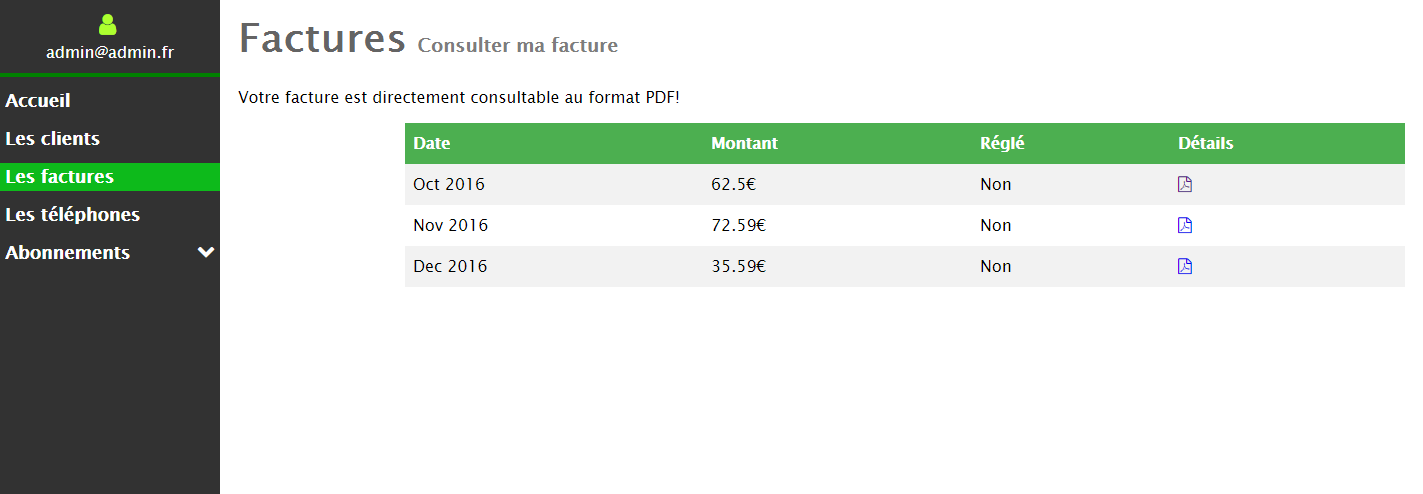
\includegraphics[width=.55\textwidth]{images/Plateforme/liste_factures}
    \caption{Liste des factures}
    \label{fig:listfacture}
\end{figure}

Les champs de ce tableau sont les suivants :
\begin{itemize}
  \itemperso{Date}Le mois de facturation : correspond à la période pendant laquelle les opérations téléphoniques ont eu lieu.
  \itemperso{Montant}Le montant de la facture à payer en euros.
  \itemperso{Reglé}\og Oui\fg si la facture est déjà payée, \og Non\fg sinon.
  \itemperso{Détails}Un lien vers une page qui génère et affiche le détails des consommations de l'utilisateur pour le mois sélectionné.
\end{itemize}

\subsubsection{Détail des consommations}

Le PDF généré donne les consommations détaillées de l'utilisateur pour trois types de consommations différentes :
\begin{itemize}
	\itemperso{SMS}Présenté en Figure~\ref{fig:liste_sms_pdf}
	\itemperso{MMS}Présenté en Figure~\ref{fig:liste_mms_pdf}
	\itemperso{appel}Présenté en Figure~\ref{fig:liste_appels_pdf}
\end{itemize}

\begin{figure}[ht]
  \begin{subfigure}{.33\textwidth}
    \centering
    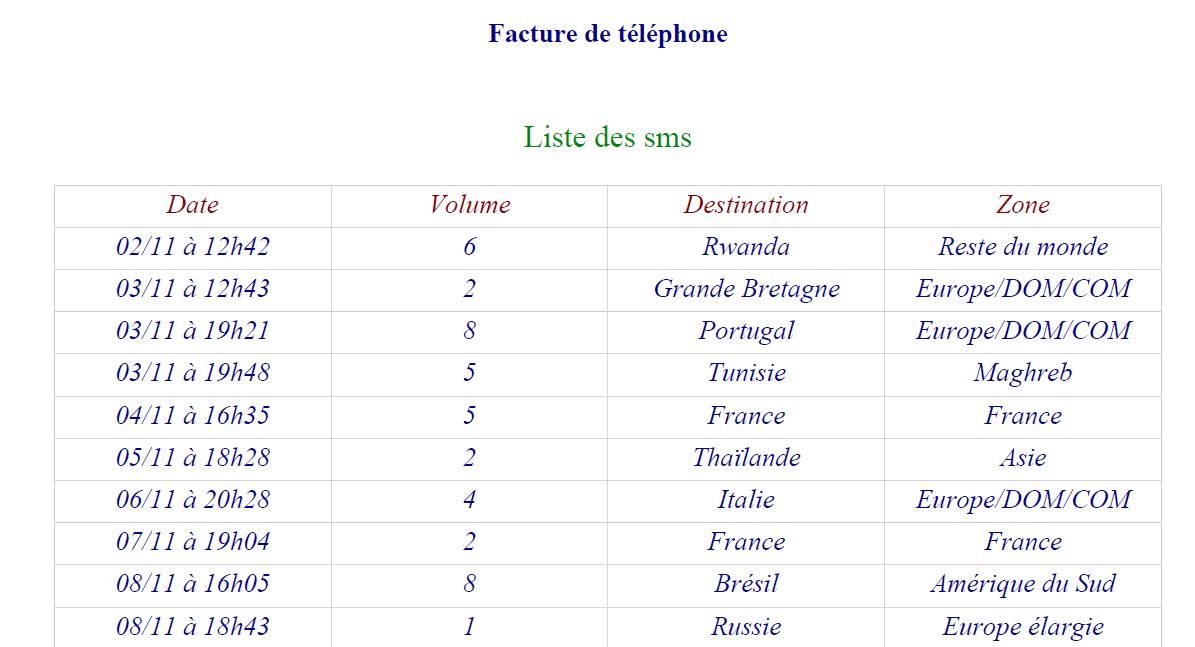
\includegraphics[width=\textwidth]{images/Plateforme/liste_sms_pdf}
    \caption{Liste des SMS}
    \label{fig:liste_sms_pdf}
  \end{subfigure}\hfill%
  \begin{subfigure}{.33\textwidth}
    \centering
    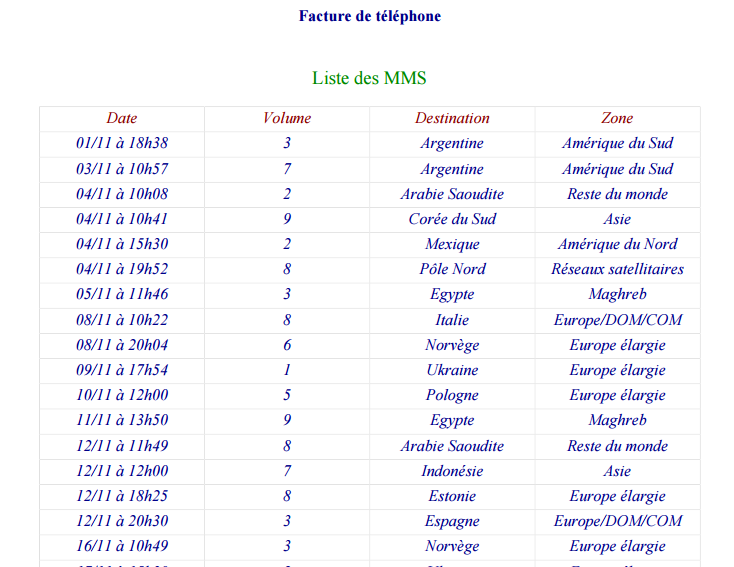
\includegraphics[width=\textwidth]{images/Plateforme/liste_mms_pdf}
    \caption{Liste des MMS}
    \label{fig:liste_mms_pdf}
  \end{subfigure}\hfill
  \begin{subfigure}{.33\textwidth}
    \centering
    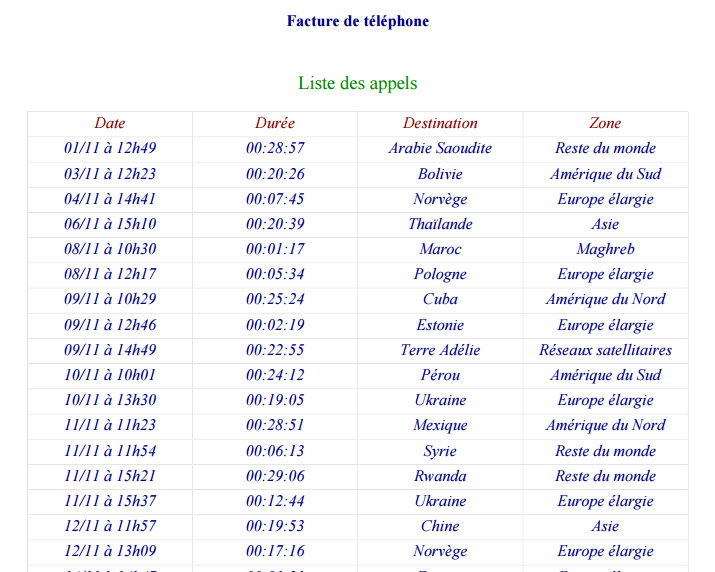
\includegraphics[width=\textwidth]{images/Plateforme/liste_appels_pdf}
    \caption{Liste des appels}
    \label{fig:liste_appels_pdf}
  \end{subfigure}
  \caption{Listes générées dans le PDF}
\end{figure}


%%% Local Variables:
%%% mode: latex
%%% TeX-master: "../../Rapport_BDD"
%%% End:
